%%%%%%%%%%%%%%%%%%%%%%%%%%%%%%%%%%%%%%%%%%%%%%%%%%%%%%%%%%%%%%%%%%%%%%
% CV – Mark Schutera
% Tufte-handout style, A4
%%%%%%%%%%%%%%%%%%%%%%%%%%%%%%%%%%%%%%%%%%%%%%%%%%%%%%%%%%%%%%%%%%%%%%
\documentclass[a4paper,notitlepage]{tufte-handout}

%%
% Packages
%%
\usepackage{graphicx}
\usepackage{booktabs}
\usepackage{xcolor}
\usepackage{enumitem}
\usepackage{microtype}
\usepackage{hyperref}
\usepackage{fontawesome5}
\usepackage{multicol}
\usepackage{array}
\usepackage{ragged2e}
\usepackage{tikz}
\usepackage{qrcode}
\usepackage{bibentry}
\usetikzlibrary{calc}

%%
% Colour palette  (design tokens)
%%
% Design tokens (from user) — clearer names
\definecolor{cv_bg}{RGB}{5,5,5}        % #000000 — Page background
\definecolor{cv_gold}{RGB}{233,196,106}   % #E9C46A — Gold/sand — headings, primary text
\definecolor{cv_orange}{RGB}{244,162,97}  % #F4A261 — Orange — secondary highlights
\definecolor{cv_burnt}{RGB}{231,111,81}   % #E76F51 — Burnt orange — tertiary text
\definecolor{cv_teal_border}{RGB}{46,90,106} % #2E5A6A — Teal border — separators
\definecolor{cv_surface}{RGB}{38,70,83}   % #264653 — Dark teal — card/surface backgrounds
\definecolor{cv_accent}{RGB}{42,157,143}   % #2A9D8F — Bright teal — accent/CTA
\definecolor{cv_text}{RGB}{196,191,185}    % #C4BFB9 — Light warm gray — body text


%%
% Hyperref setup
%%
\hypersetup{
  colorlinks=true,
  urlcolor=cv_accent,
  linkcolor=cv_accent
}

%%
% Suppress section numbering
%%
\setcounter{secnumdepth}{-1}

%%
% Custom commands
%%
\newcommand{\monthyear}{March 2026}
\newcommand{\faicon}[1]{{\color{cv_orange}#1}}

% CV entry: #1=title, #2=dates, #3=employer, #4=location
\newcommand{\cventry}[4]{%
  \marginnote{\footnotesize\color{cv_orange}\textit{#2}\\[2pt]\color{cv_burnt}\textsc{#3}\\[1pt]#4}%
  \noindent{\color{cv_gold}\textsc{\large #1}}\par\nobreak
}


%%
% Document
%%
%%
% Black background on every page (TikZ, no extra package needed)
%%
\AddToHook{shipout/background}{%
  \put(0,-\paperheight){%
    \color{cv_bg}\rule{\paperwidth}{\paperheight}}%
}

\begin{document}
\bibliographystyle{plainnat}
\nobibliography{references}
\color{cv_text}
\pagestyle{empty}

%%------------------------------------------------------------------------
%% PHOTO — page overlay, flush top-right, diagonal lower-left cut
%%------------------------------------------------------------------------
\begin{tikzpicture}[remember picture, overlay]
  \begin{scope}
    \clip (current page.north east)
          -- ++(-9.5cm,  0)
          -- ++(0,      -5.0cm)
          -- ++(3.5cm,  -3.0cm)
          -- ++(6.0cm,   0)
          -- cycle;
    \node[anchor=north east, inner sep=0pt, opacity=0.35] at (current page.north east)
      {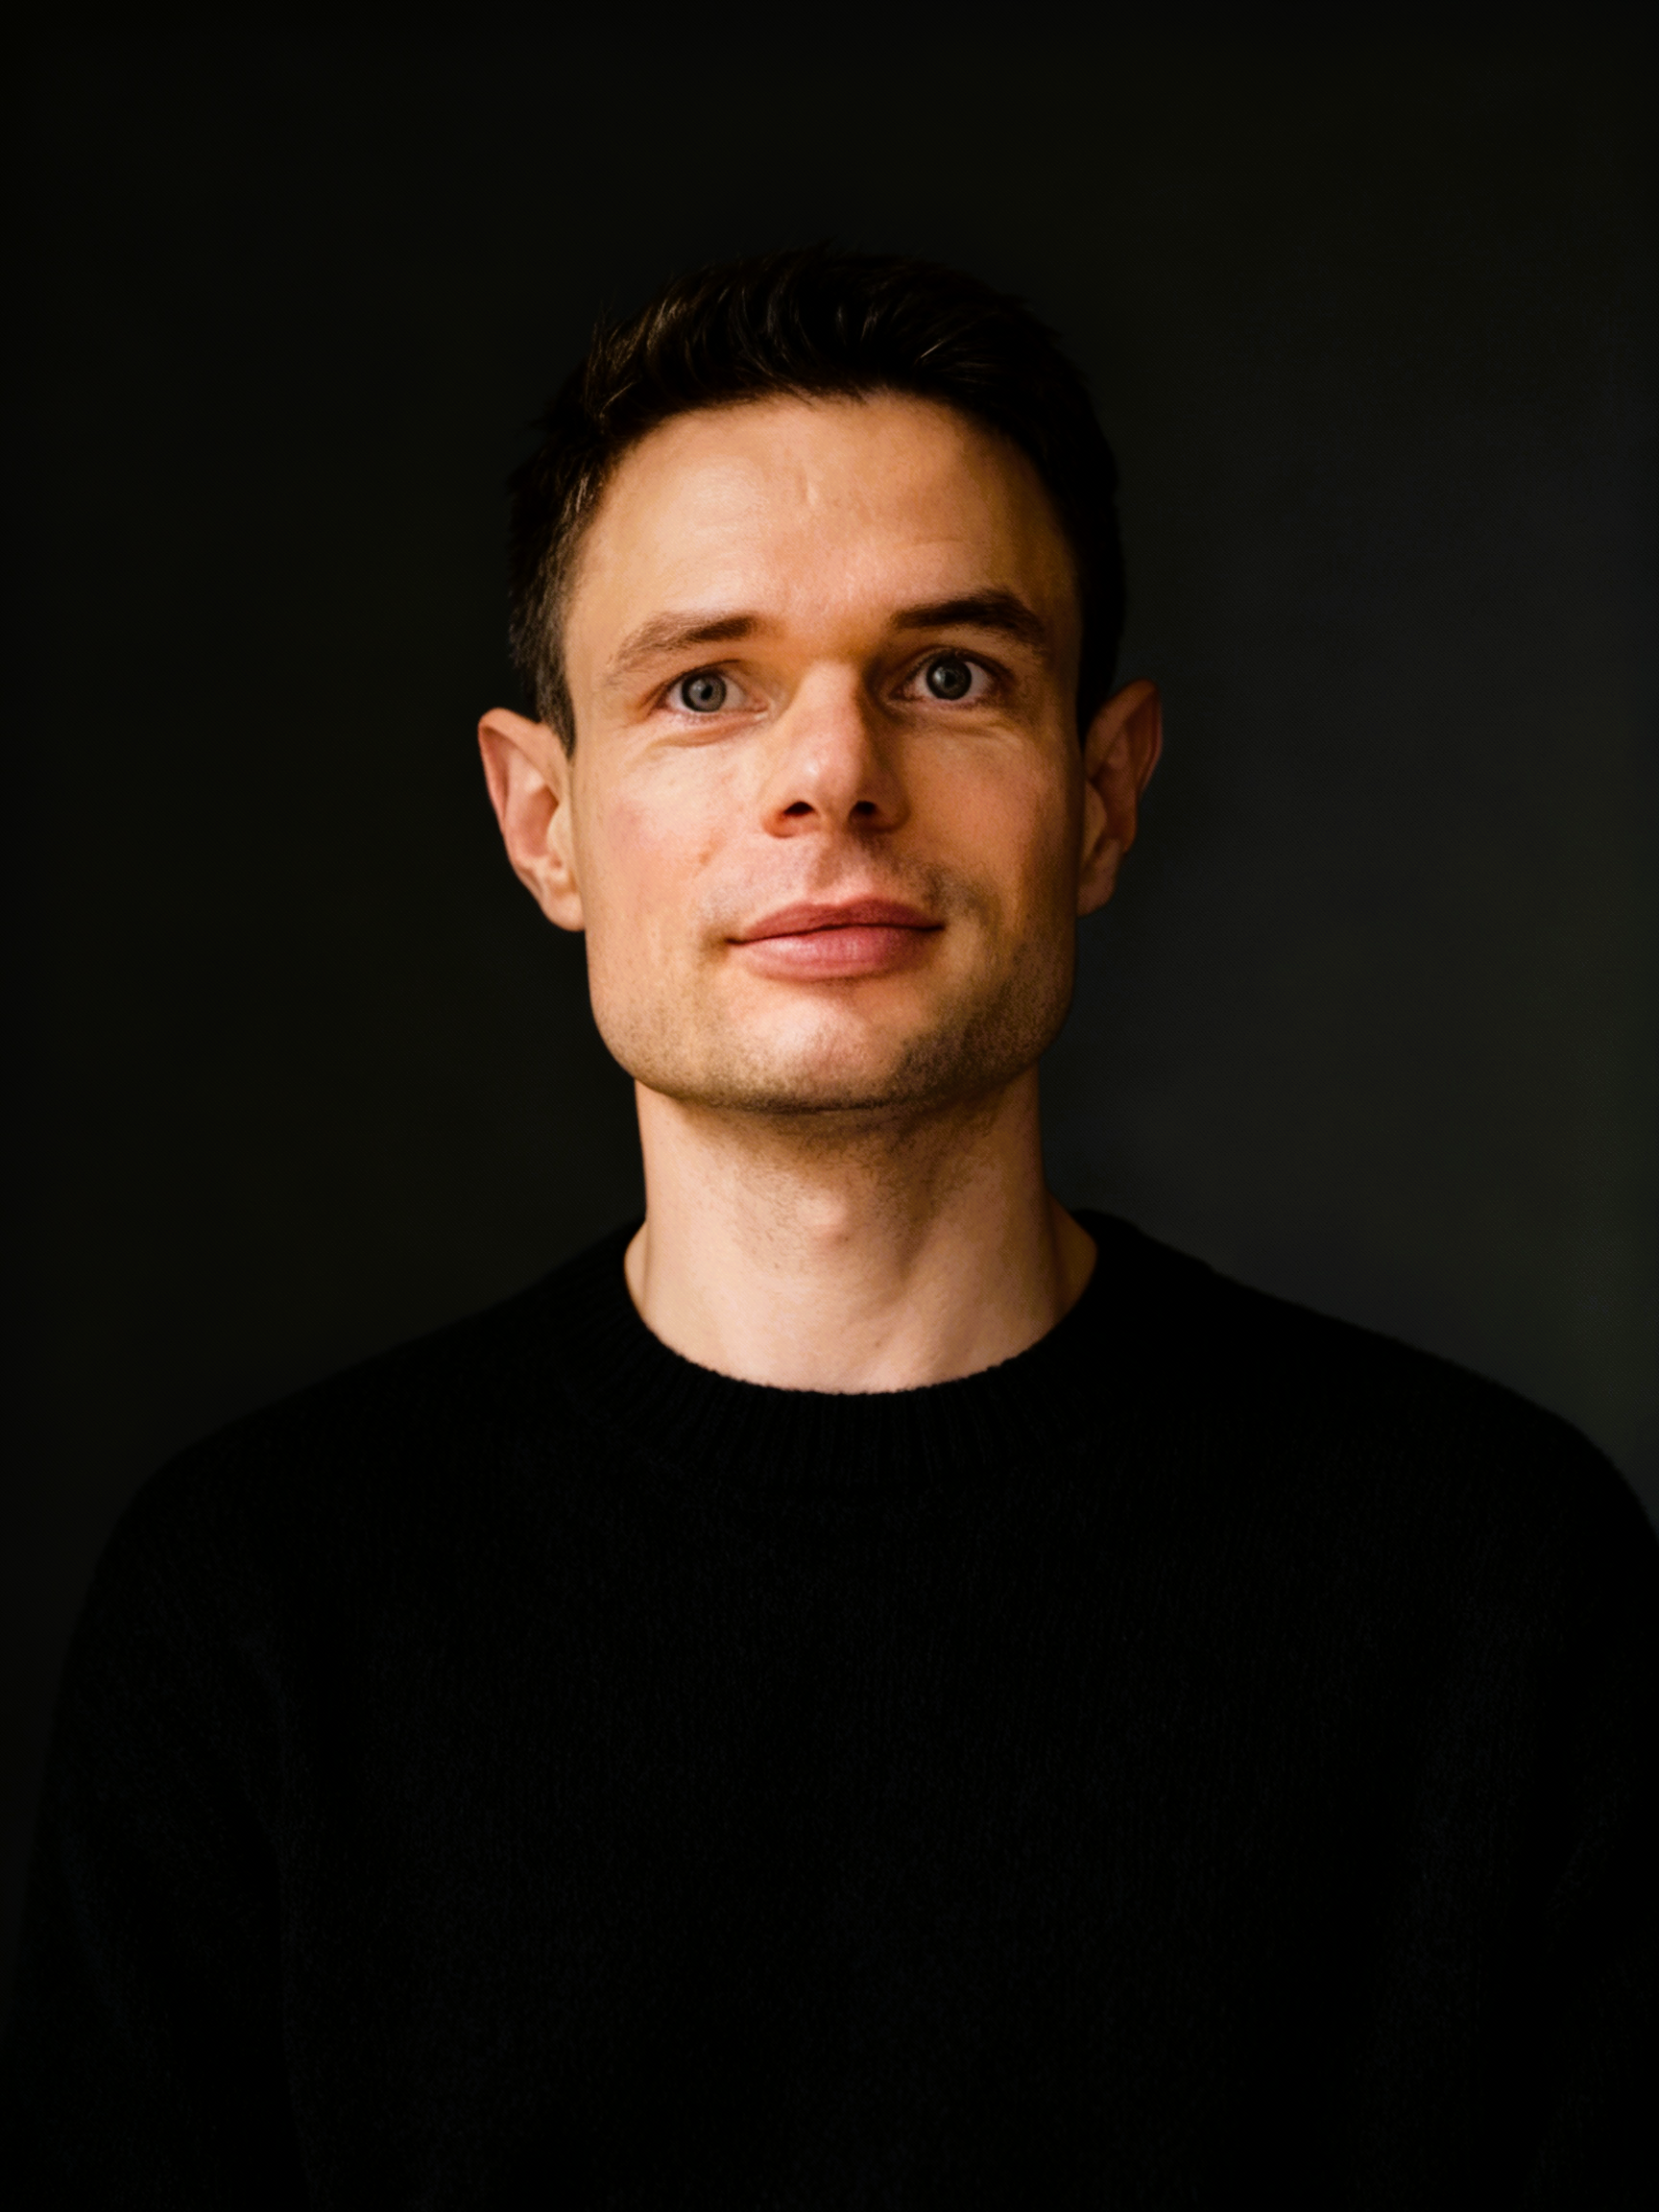
\includegraphics[height=10.5cm]{profilemark_punch.png}};
  \end{scope}
\end{tikzpicture}

%%------------------------------------------------------------------------
%% HEADER (fullwidth)
%%------------------------------------------------------------------------
\begin{fullwidth}
\noindent
\begin{minipage}[t]{0.52\linewidth}
  \vspace{0pt}
  {\fontsize{28}{30}\selectfont\color{cv_accent}\textsc{\href{mailto:mark@schutera.com}{Mark Schutera}}}\par
  \medskip
    {\large\color{cv_gold} Prof. Dr.-Ing. Artificial Intelligence}\par


  \iffalse
  \bigskip
  \begin{tabular}{@{}ll}
    \faicon{\faMapMarker*}    & {\color{cv_accent}Am Bl\"{a}siberg 18, 88250 Weingarten, Germany} \\[3pt]
    \faicon{\faEnvelope}      & \href{mailto:Mark.schutera@mailbox.org}{mark.schutera@mailbox.org} \\[3pt]
    \faicon{\faPhone}         & {\color{cv_accent}+49\,1520\,713\,7061} \\[3pt]
  \end{tabular}
  \fi
\end{minipage}
\end{fullwidth}

\vspace{1.8em}


% ---- Professor DHBW (current) ----
\cventry{}{04.2026 -- present}{DHBW (Cooperative State University)}{Ravensburg, Germany}
\marginnote{%
  \flushright
  {\color{cv_surface}\qrcode[height=0.9cm]{https://scholar.google.com/citations?user=jFrk3WoAAAAJ&hl=de}}\\[4pt]
  {\footnotesize \faicon{\faGraduationCap}\ \href{https://scholar.google.com/citations?user=jFrk3WoAAAAJ&hl=de}{{\color{cv_gold}Google Scholar h-index 10}}}
}%
% my most cited paper, paper with most momentum, and most recent paper.

\newthought{Teaching and research in artificial intelligence} with a focus on machine learning, 
deep learning, computer vision and embodied AI. Responsible for student development, lecture design 
and supervision of industrial cooperations in applied AI.


\vspace{1.8em}

% ---- Head of Industrial AI ----
\cventry{Managing Director}{01.2025 -- present}{Schutera UG}{Remote, Germany}
\marginnote{%
  \flushright
  {\color{cv_surface}\qrcode[height=0.9cm]{https://github.com/schutera}}\\[4pt]
  {\footnotesize \faicon{\faGithub}\ \href{https://github.com/schutera}{{\color{cv_gold} My GitHub profile}}}
}
\newthought{Consulting on} AI vision and strategy, prototyping and product development, workshops and key-notes.

\section*{\color{cv_accent}Prior Experience}
\noindent{\color{cv_accent}\rule{\linewidth}{0.6pt}}\vspace{4pt}

% ---- Head of Industrial AI ----
\cventry{Head of Industrial AI Global Operations}{02.2024 -- 03.2026}{ZF LIFETEC}{Remote, Germany}
{\footnotesize\textsc{\color{cv_teal_border} Strategy \textbullet{} MLOps \& LLMOps \textbullet{} Industrial Automation \textbullet{} 
Scaled Infrastructure \textbullet{} Agile Project Management \textbullet{} Vision}}
\marginnote{%
  \flushright
  {\color{cv_surface}\qrcode[height=0.9cm]{https://www.linkedin.com/feed/update/urn:li:activity:7399032874345340929/}}\\[4pt]
  {\footnotesize \faicon{\faLinkedin}\ \href{https://www.linkedin.com/feed/update/urn:li:activity:7399032874345340929/}{{\color{cv_gold} AI Strategy Clip on my LinkedIn}}}
}
\newthought{Built and led a global team} of AI Architects and MLOps Engineers. 
Responsible for global AI operations strategy, from organizational structure, vision, and adoption, through full-stack AI architecture for AI agents and centralized MLOps platforms.


\vspace{1.8em}

\cventry{Team Lead Autonomous Driving Software}{02.2020 -- 02.2024}{ZF Friedrichshafen AG}{Friedrichshafen, Germany}
{\footnotesize\textsc{\color{cv_teal_border} AD Software Validation \textbullet{} iSAQB Software Architect \textbullet{} Leadership in distributed Teams \textbullet{} UX \& UI \textbullet{} AI Product Management \textbullet{} Scrum PSPO II }}
\marginnote{%
  \flushright
  {\color{cv_surface}\qrcode[height=0.9cm]{https://patents.google.com/?inventor=Mark+Schutera}}\\[4pt]
  {\footnotesize \faicon{\faPaper}\ \href{https://patents.google.com/?inventor=Mark+Schutera}{{\color{cv_gold} 50+ patents with the DPMA}}}
}

\newthought{Led a software engineering team}; Product Owner of the perception ML stack and validation tooling. Drove development of ZF's high-performance ML compute cluster.

\vspace{1.8em}

% ---- Machine Learning Engineer ----
\cventry{Machine Learning Engineer}{09.2017 -- 01.2020}{ZF Friedrichshafen AG}{Friedrichshafen, Germany}
{\footnotesize\textsc{\color{cv_teal_border} Deep Learning \& Computer Vision \textbullet{} Python \textbullet{} PyTorch \& Tensorflow \textbullet{} 
B1 Test Driver License BMW \textbullet{} ISTQB Software Tester}} \\

\cventry{}{08.2018 -- 05.2019}{ZF Innovation Hub}{Sunnyvale, USA}
\marginnote{\newthought{10-month research stay at the UC Berkely} Deep Driving Consortium.
}

\marginnote{\flushright\footnotesize\color{cv_accent} English~
\begin{tikzpicture}[scale=0.5, baseline=-0.5ex]
  \foreach \i in {1,...,4} {
    \fill[cv_accent] (\i*0.7,0) circle (0.3);
  }
  \foreach \i in {5} {
    \draw[cv_accent, line width=0.8pt] (\i*0.7,0) circle (0.3);
  }
\end{tikzpicture}
}

\newthought{R\&D of automotive vision algorithms} in cooperation with KIT (PhD-affiliated). Focus on continuous integration and unsupervised domain adaptation of deep learning models. Organised the ZF ML Colloquium; supervised student research teams.




\vspace{1.8em}

% ---- SAP ----
\cventry{Junior Research Fellow Deep Learning}{06.2017 -- 08.2017}{SAP Israel Innovation Center}{Tel Aviv, Israel}
{\footnotesize\textsc{\color{cv_teal_border} Rapid Prototyping \textbullet{} Python \& TensorFlow \textbullet{} Algorithm Development 
\textbullet{} Neural Networks \textbullet{} Edge AI}} \\
\marginnote{\flushright\footnotesize\color{cv_accent} Russian (A1)~
\begin{tikzpicture}[scale=0.5, baseline=-0.5ex]
  \foreach \i in {1} {
    \fill[cv_accent] (\i*0.7,0) circle (0.3);
  }
  \foreach \i in {2,3,4,5} {
    \draw[cv_accent, line width=0.8pt] (\i*0.7,0) circle (0.3);
  }
\end{tikzpicture}

}
\marginnote{%
  \flushright
  {\color{cv_surface}\qrcode[height=0.9cm]{https://stackoverflow.com/users/5763590/mrk}}\\[4pt]
  {\footnotesize \faicon{\faStackOverflow}\ \href{https://stackoverflow.com/users/5763590/mrk}{{\color{cv_gold} Stack Overflow >10k reps}}}
}
\newthought{3-month R\&D within SAP's deep learning team.} Development and training of neural networks for video and time-series analysis; prototyped and prepared models for edge devices.

\vspace{1.8em}

% ---- KUKA ----
\cventry{Student Researcher Robotics}{10.2016 -- 05.2017}{KUKA Robotics Corporate Research}{Augsburg, Germany}
{\footnotesize\textsc{\color{cv_teal_border} Robotics \textbullet{} LBR iiwa Cobot \textbullet{} ROS \textbullet{} OpenCV \textbullet{} Unsupervised Learning \& Active Vision}} \\
\newthought{8-month internship and thesis work}\cite{KUKA_Patent} within the machine learning group. 
Research and development of unsupervised object recognition and active vision
on the KUKA Cobot LBR iiwa.



\vspace{1.8em}


%%------------------------------------------------------------------------
%% EDUCATION
%%------------------------------------------------------------------------
\noindent{\color{cv_accent}\rule{\linewidth}{0.6pt}}\vspace{4pt}


% ---- PhD ----
\cventry{Dr.-Ing.\ (PhD)}{09.2017 -- 09.2023}{Karlsruhe Institute of Technology}{}
{\footnotesize\textsc{\color{cv_teal_border} Summa cum laude}} 

\newthought{Dissertation on unsupervised domain adaptation}\cite{DoctoralThesis} 
for cognitive perception systems. Programme committee for CVPR and NeurIPS workshops. 
KHYS Networking Grant 2020 (ETH Zurich); ZF Excellence Award 2019; KI-Newcomer 2019 (Top~50).

\vspace{1.8em}

% ---- MSc ----
\cventry{M.Sc.\ Cognitive Technical Systems}{08.2015 -- 05.2017}{KIT}{}
\newthought{Focus} on cognitive technical systems and robotics\cite{BSc_Publication}. 
Instructor for mechanical design (KIT/IPEK); research assistant for image and data analysis (KIT/IAI); KIT Award for Outstanding Student Research; Hans Voith Award.

\vspace{1.8em}

% ---- BSc ----
\cventry{B.Sc. Mechanical Engineering}{09.2011 -- 08.2015}{KIT}{}

\cventry{}{09.2013 -- 05.2014}{KTH Royal Institute of Technology}{Stockholm, Sweden}

\marginnote{\newthought{Two-term Erasmus Exchange.} Head of the German Language Caf\'{e} at KTH.
}
\newthought{Focus} on control information technology, computer vision and automation.
\marginnote{\flushright\footnotesize\color{cv_accent} Swedish (B1)~
\begin{tikzpicture}[scale=0.5, baseline=-0.5ex]
  \foreach \i in {1,...,3} {
    \fill[cv_accent] (\i*0.7,0) circle (0.3);
  }
  \foreach \i in {4,5} {
    \draw[cv_accent, line width=0.8pt] (\i*0.7,0) circle (0.3);
  }
\end{tikzpicture}
}



\cventry{}{08.2010 -- 07.2011}{German Red Cross (DRK)}{Hohenlohe, Germany}
\marginnote{\newthought{Paramedic.} Social year in emergency-medical 
and technical rescue. High-pressure decision-making.}

\marginnote{\flushright\footnotesize\color{cv_accent} German~
\begin{tikzpicture}[scale=0.5, baseline=-0.5ex]
  \foreach \i in {1,...,5} {
    \fill[cv_accent] (\i*0.7,0) circle (0.3);
  }
\end{tikzpicture}
}
\marginnote{\flushright\footnotesize\color{cv_accent} French (A2)~
\begin{tikzpicture}[scale=0.5, baseline=-0.5ex]
  \foreach \i in {1,2} {
    \fill[cv_accent] (\i*0.7,0) circle (0.3);
  }
  \foreach \i in {3,4,5} {
    \draw[cv_accent, line width=0.8pt] (\i*0.7,0) circle (0.3);
  }
\end{tikzpicture}
}


\vspace{1.8em}
\vspace{1.8em}

\noindent
\includegraphics[width=8cm]{signature_inverted.png}

\vspace{-2.5em}
\noindent Prof. Dr.-Ing.\ Mark Schutera \\
\noindent Weingarten, \monthyear


\end{document}
